\begin{frame} {Definition of a manipulation planning problem}
  \parbox{.39\linewidth} {
    \begin{itemize}
    \item grippers (frames attached to a joint),
    \item handles (frames attached to a joint),
    \item contact surfaces
    \end{itemize}
    define grasps and stable poses for objects.
  }
  \parbox{.59\linewidth} {
    \begin{center}
      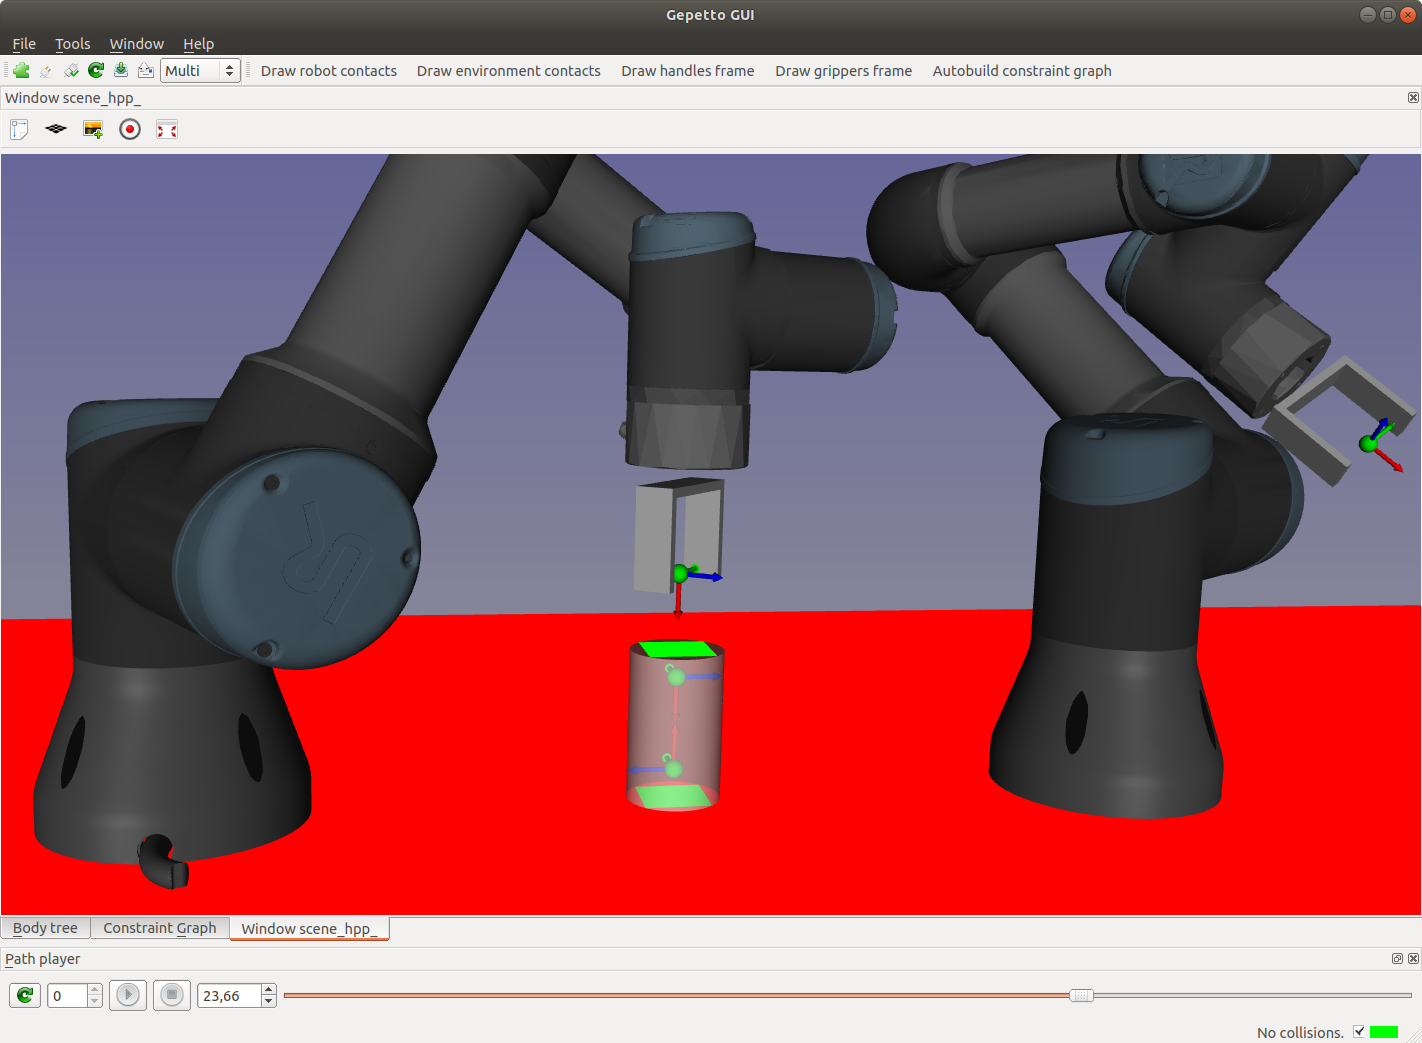
\includegraphics[width=\linewidth]{figures/manipulation-problem.png}
    \end{center}
  }
\end{frame}

\begin{frame} {The factory}
  \parbox{.39\linewidth} {
  Given all the possible grasps (defined by grippers and handle), a factory builds the constraint
  graph with all possible states
  }
  \parbox{.59\linewidth} {
    \begin{center}
      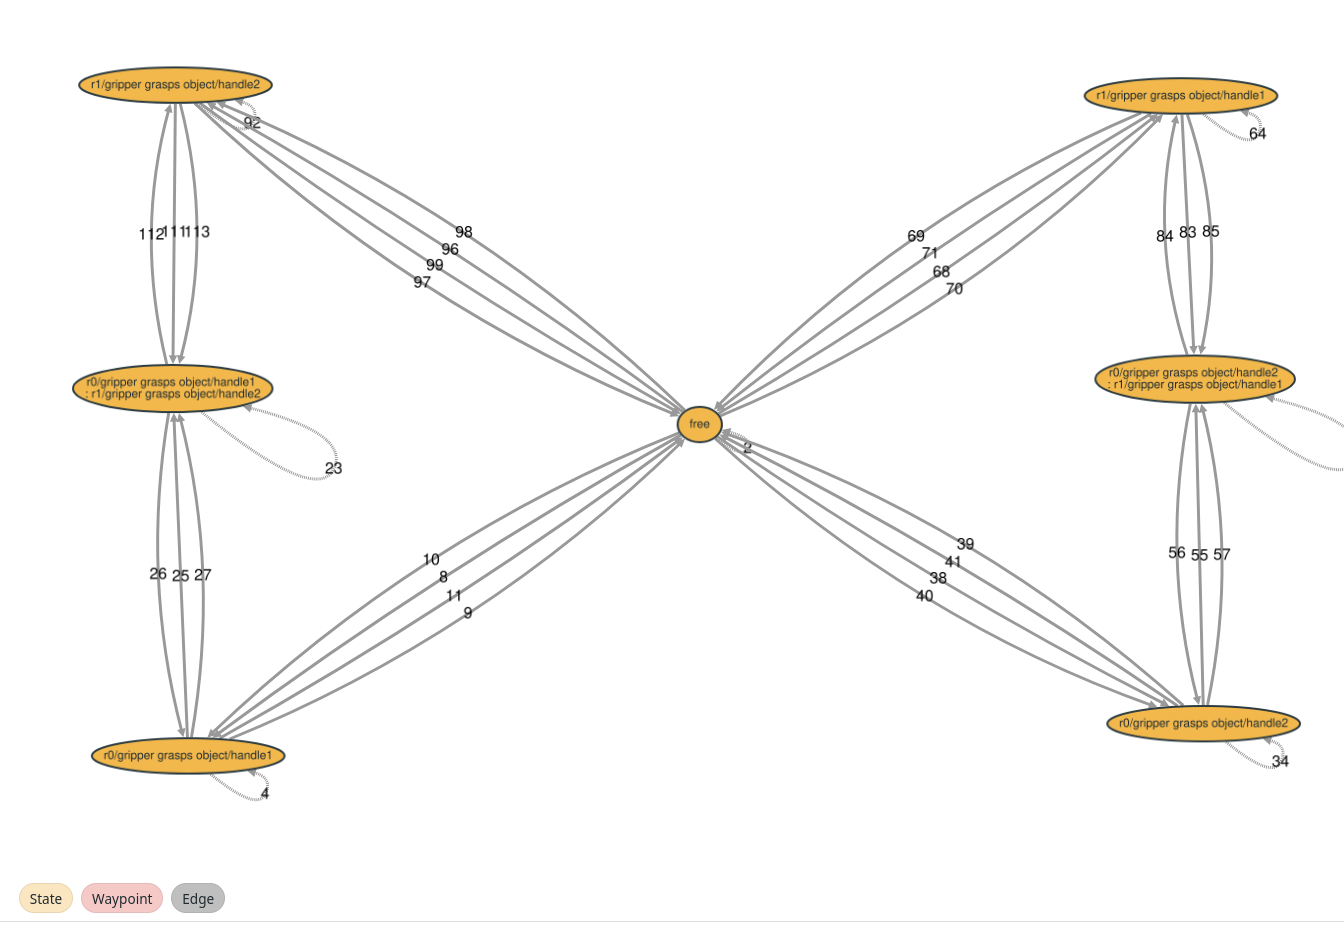
\includegraphics[width=\linewidth]{figures/constraint-graph-raw.png}
    \end{center}
  }
\end{frame}

\begin{frame} {Waypoint transitions and states}
  \parbox{.59\linewidth} {
    To ease manipulation planning resolution, some intermediate states are inserted by the factory.
  }
  \parbox{.39\linewidth} {
    \begin{center}
      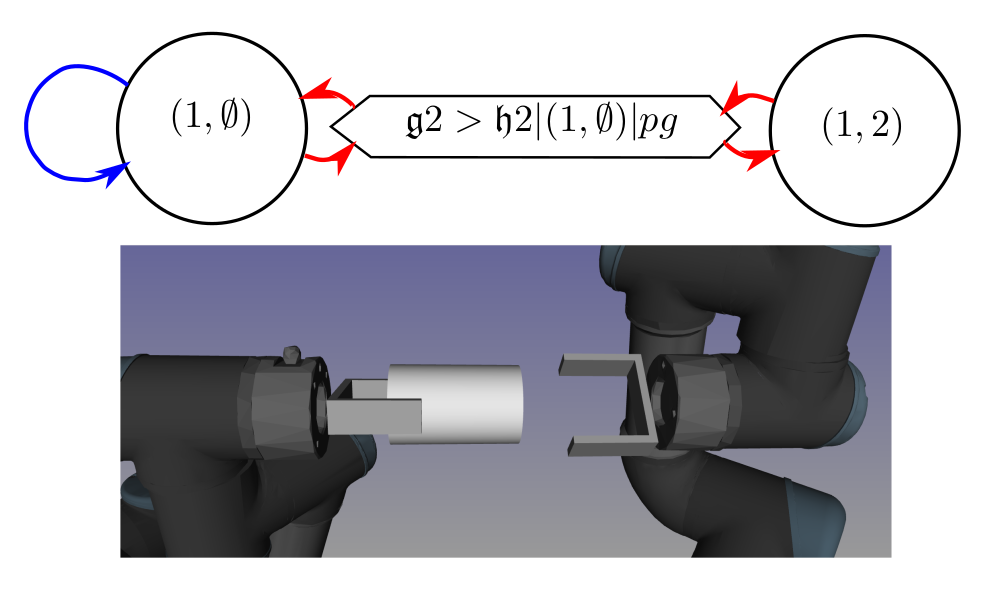
\includegraphics[width=\linewidth]{figures/waypoint-1.png}
      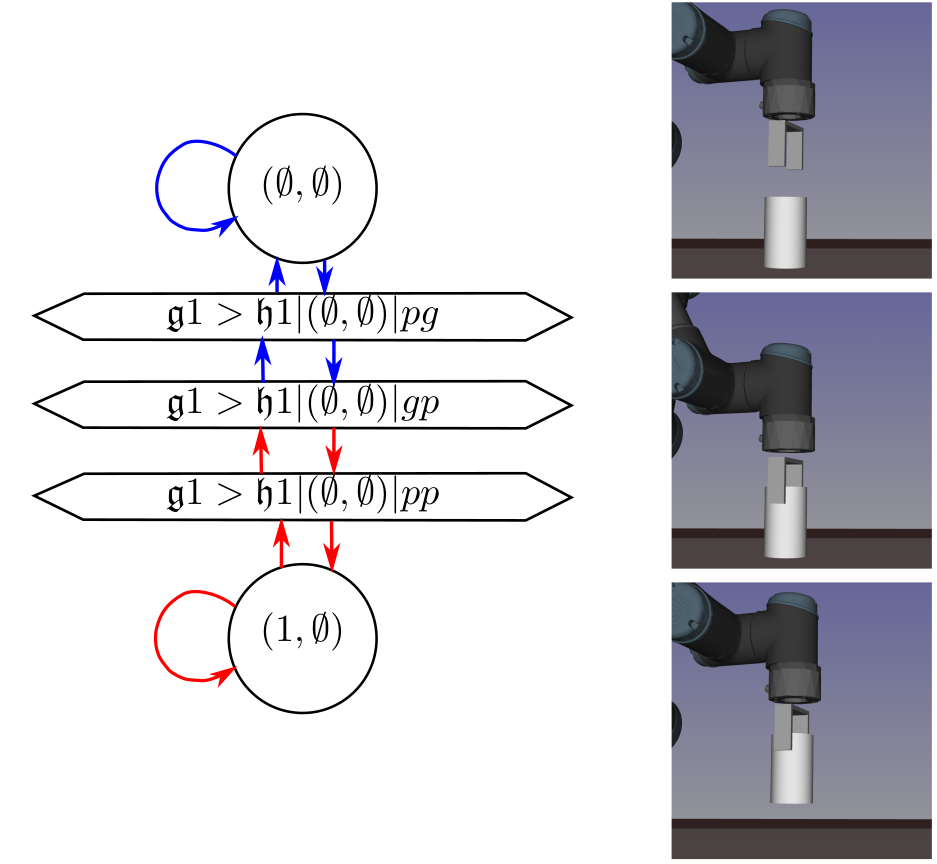
\includegraphics[width=\linewidth]{figures/waypoints-3.png}
    \end{center}
  }
\end{frame}

\begin{frame} {Waypoint transitions and states}
  \begin{center}
    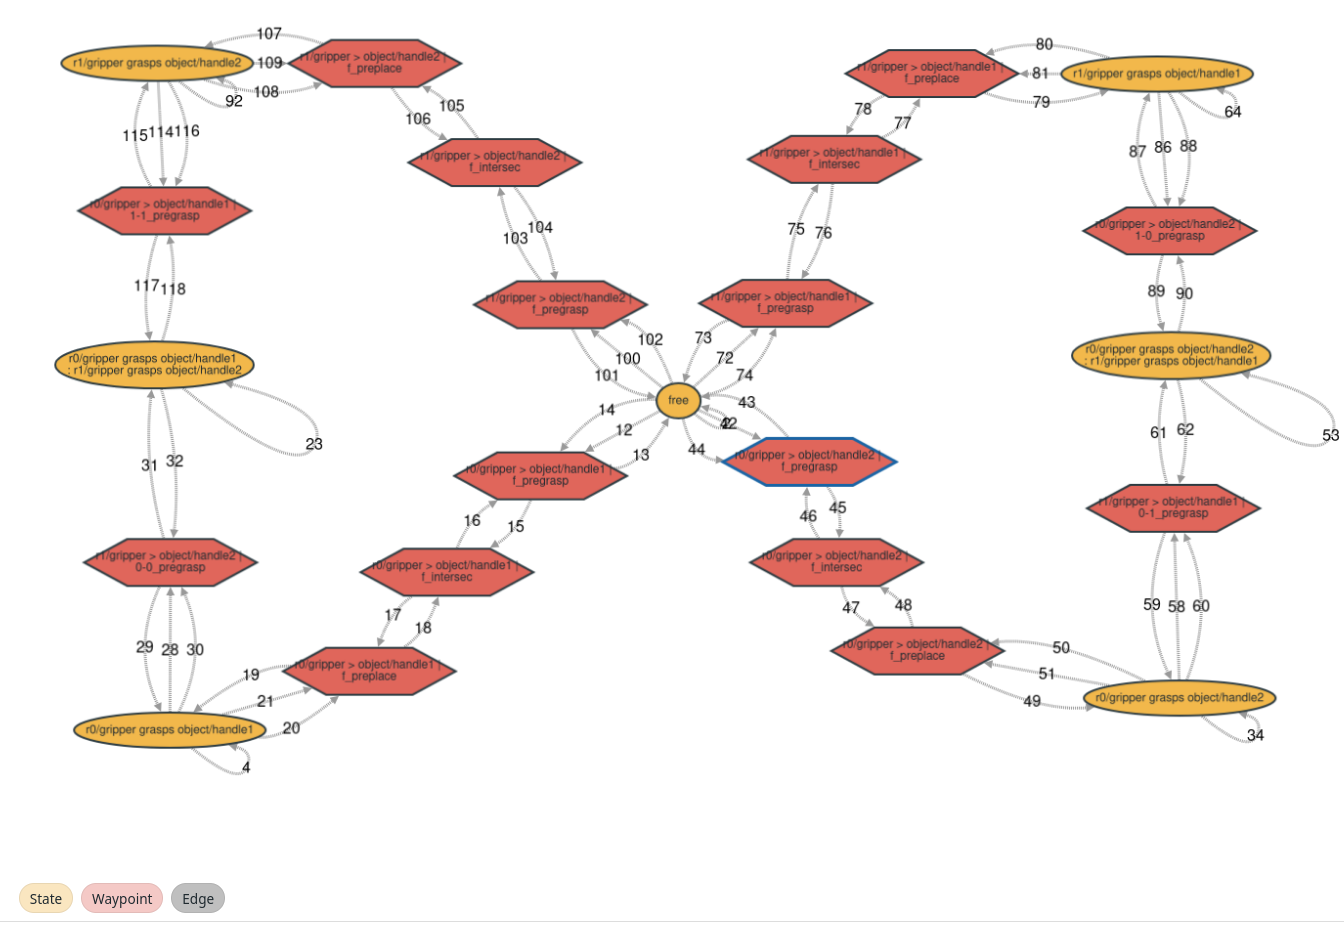
\includegraphics[width=.9\linewidth]{figures/constraint-graph-waypoints.png}
  \end{center}
\end{frame}

\begin{frame} {Resources}
  \begin{itemize}
  \item \href{https://laas.hal.science/LAAS-GEPETTO/hal-02995125v2}{F.~Lamiraux and J.~Mirabel, Prehensile Manipulation Planning: Modeling, Algorithms and Implementation, IEEE transactions on Robotics, 2022},
  \item \href{https://humanoid-path-planner.github.io/hpp-doc}{Online documentation}
  \end{itemize}
\end{frame}
